\documentclass[11pt,compress,t,notes=noshow, xcolor=table]{beamer}
\usepackage[]{graphicx}\usepackage[]{color}
% maxwidth is the original width if it is less than linewidth
% otherwise use linewidth (to make sure the graphics do not exceed the margin)
\makeatletter
\def\maxwidth{ %
  \ifdim\Gin@nat@width>\linewidth
    \linewidth
  \else
    \Gin@nat@width
  \fi
}
\makeatother

\definecolor{fgcolor}{rgb}{0.345, 0.345, 0.345}
\newcommand{\hlnum}[1]{\textcolor[rgb]{0.686,0.059,0.569}{#1}}%
\newcommand{\hlstr}[1]{\textcolor[rgb]{0.192,0.494,0.8}{#1}}%
\newcommand{\hlcom}[1]{\textcolor[rgb]{0.678,0.584,0.686}{\textit{#1}}}%
\newcommand{\hlopt}[1]{\textcolor[rgb]{0,0,0}{#1}}%
\newcommand{\hlstd}[1]{\textcolor[rgb]{0.345,0.345,0.345}{#1}}%
\newcommand{\hlkwa}[1]{\textcolor[rgb]{0.161,0.373,0.58}{\textbf{#1}}}%
\newcommand{\hlkwb}[1]{\textcolor[rgb]{0.69,0.353,0.396}{#1}}%
\newcommand{\hlkwc}[1]{\textcolor[rgb]{0.333,0.667,0.333}{#1}}%
\newcommand{\hlkwd}[1]{\textcolor[rgb]{0.737,0.353,0.396}{\textbf{#1}}}%
\let\hlipl\hlkwb

\usepackage{framed}
\makeatletter
\newenvironment{kframe}{%
 \def\at@end@of@kframe{}%
 \ifinner\ifhmode%
  \def\at@end@of@kframe{\end{minipage}}%
  \begin{minipage}{\columnwidth}%
 \fi\fi%
 \def\FrameCommand##1{\hskip\@totalleftmargin \hskip-\fboxsep
 \colorbox{shadecolor}{##1}\hskip-\fboxsep
     % There is no \\@totalrightmargin, so:
     \hskip-\linewidth \hskip-\@totalleftmargin \hskip\columnwidth}%
 \MakeFramed {\advance\hsize-\width
   \@totalleftmargin\z@ \linewidth\hsize
   \@setminipage}}%
 {\par\unskip\endMakeFramed%
 \at@end@of@kframe}
\makeatother

\definecolor{shadecolor}{rgb}{.97, .97, .97}
\definecolor{messagecolor}{rgb}{0, 0, 0}
\definecolor{warningcolor}{rgb}{1, 0, 1}
\definecolor{errorcolor}{rgb}{1, 0, 0}
\newenvironment{knitrout}{}{} % an empty environment to be redefined in TeX

\usepackage{alltt}
\newcommand{\SweaveOpts}[1]{}  % do not interfere with LaTeX
\newcommand{\SweaveInput}[1]{} % because they are not real TeX commands
\newcommand{\Sexpr}[1]{}       % will only be parsed by R



\usepackage[english]{babel}
\usepackage[utf8]{inputenc}

\usepackage{dsfont}
\usepackage{verbatim}
\usepackage{amsmath}
\usepackage{amsfonts}
\usepackage{bm}
\usepackage{csquotes}
\usepackage{multirow}
\usepackage{longtable}
\usepackage{booktabs}
\usepackage{enumerate}
\usepackage[absolute,overlay]{textpos}
\usepackage{psfrag}
\usepackage{algorithm}
\usepackage{algpseudocode}
\usepackage{eqnarray}
\usepackage{arydshln}
\usepackage{tabularx}
\usepackage{placeins}
\usepackage{tikz}
\usepackage{setspace}
\usepackage{colortbl}
\usepackage{mathtools}
\usepackage{wrapfig}
\usepackage{bm}
\usetikzlibrary{shapes,arrows,automata,positioning,calc,chains,trees, shadows}
\tikzset{
  %Define standard arrow tip
  >=stealth',
  %Define style for boxes
  punkt/.style={
    rectangle,
    rounded corners,
    draw=black, very thick,
    text width=6.5em,
    minimum height=2em,
    text centered},
  % Define arrow style
  pil/.style={
    ->,
    thick,
    shorten <=2pt,
    shorten >=2pt,}
}
\usepackage{subfig}


% Defines macros and environments
\input{../../style/common.tex}

%\usetheme{lmu-lecture}
\newcommand{\titlefigure}{figure_man/roc-mannwhitney2.png}
\newcommand{\learninggoals}{
\item Understand the rank-based nature of AUC
\item See the connection between AUC and Mann-Whitney-U statistic}
\usepackage{../../style/lmu-lecture}

\let\code=\texttt
\let\proglang=\textsf

\setkeys{Gin}{width=0.9\textwidth}

\title{Introduction to Machine Learning}
% \author{Bernd Bischl, Christoph Molnar, Daniel Schalk, Fabian Scheipl}
\institute{\href{https://compstat-lmu.github.io/lecture_i2ml/}{compstat-lmu.github.io/lecture\_i2ml}}
\date{}

\setbeamertemplate{frametitle}{\expandafter\uppercase\expandafter\insertframetitle}


\begin{document}


% This file loads R packages, configures knitr options and sets preamble.Rnw as parent file
% IF YOU MODIFY THIS, PLZ ALSO MODIFY setup.Rmd ACCORDINGLY...


% Defines macros and environments
\input{../../latex-math/basic-math.tex}
\input{../../latex-math/basic-ml.tex}
\input{../../latex-math/ml-automl.tex}
%! includes: basics-learners 

\lecturechapter{Evaluation: AUC \& Mann-Whitney-U Test}
\lecture{Introduction to Machine Learning}

% ------------------------------------------------------------------------------

\begin{vbframe}{AUC as a rank-based metric}

\begin{itemize}
  \item The AUC metric is intimately related to the \textbf{Mann-Whitney-U 
  test}, also known as \textbf{Wilcoxon rank-sum test}.
  \item This connection is best understood viewing the AUC from a slightly 
  different angle: it is, in effect, a \textbf{rank-based} metric.
  \item Recall that, constructing the ROC curve, we count TP and FP.
  \begin{center}
  \includegraphics[trim = 0 0 0 -20, clip, width=0.5\textwidth]
  {figure/eval_mclass_roc_sp_12_1} 
  \end{center}
  \item The AUC abstracts from the actual classification scores and
  considers only their rank.
\end{itemize}

\framebreak 

\begin{itemize}
  \small
  \item We can interpret the AUC as the probability of our classifier 
  ranking a random positive observation higher than a random negative one.
  \item A perfect classifier will rank all positive above all negative 
  observations, achieving AUC = 1.
\end{itemize}

\begin{center}
% FIGURE SOURCE: https://docs.google.com/drawings/d/1flfi73s8qr53-ZE6oq4qRGIG-sccpBp2cSfw1Stxh8I/edit
  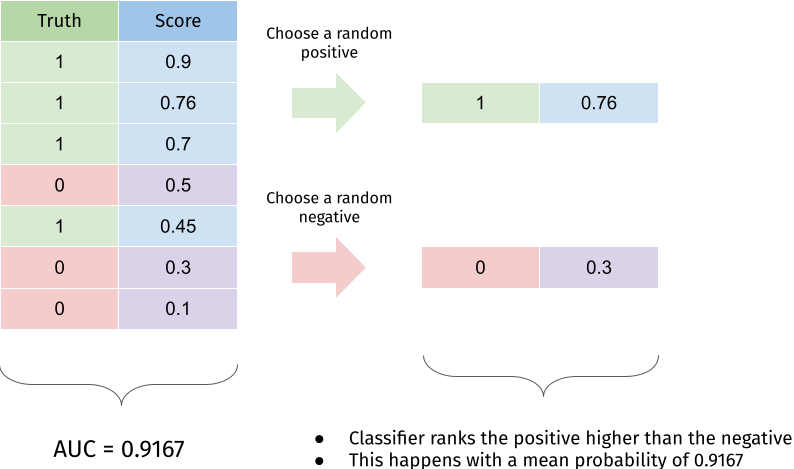
\includegraphics[width=0.55\textwidth]{figure_man/auc_interpretation_new}
  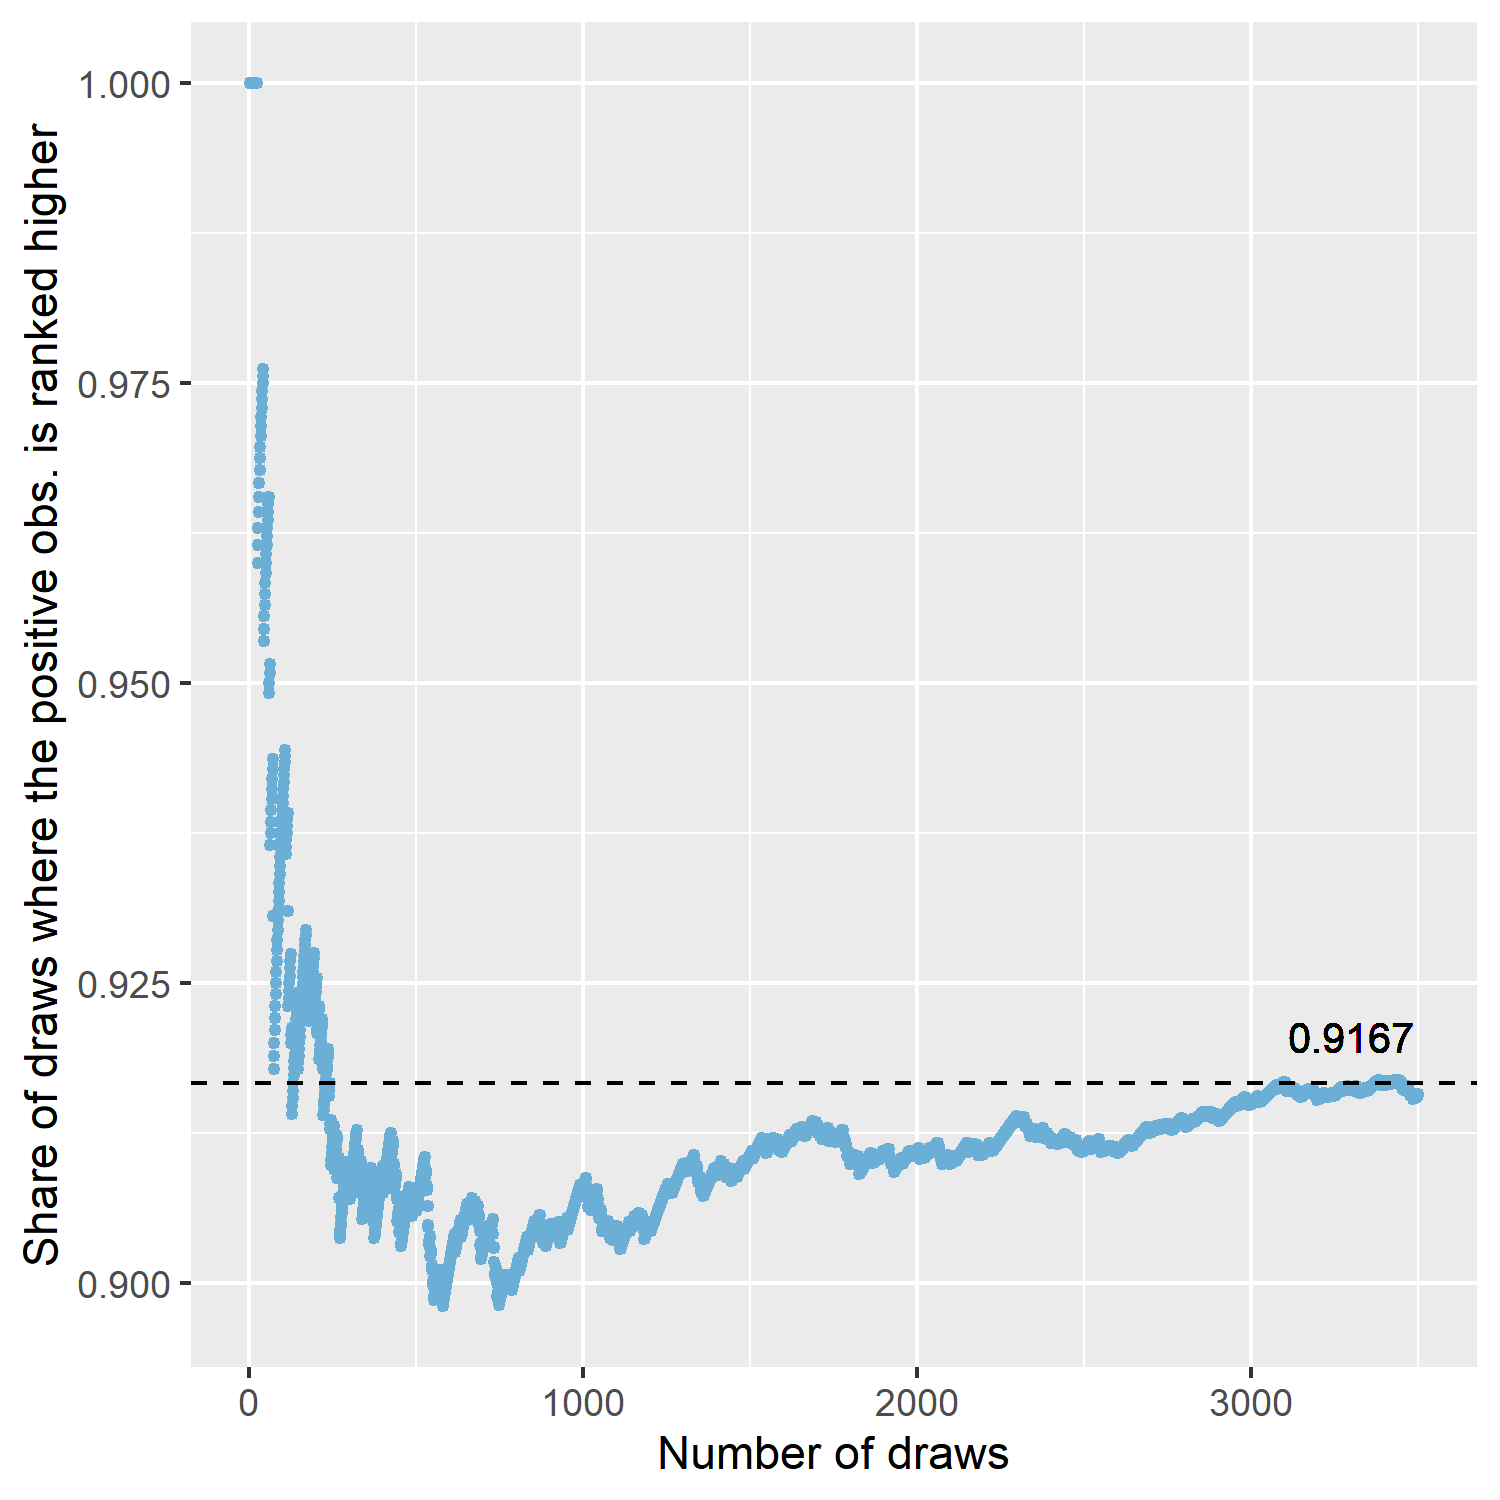
\includegraphics[width=0.4\textwidth] {figure/fig-eval_mwu_ranking}
\end{center}

\end{vbframe}

% ------------------------------------------------------------------------------

\begin{vbframe}{Mann-Whitney-U test}

\begin{itemize}
  \item The Mann-Whitney-U test is a \textbf{non-parametric hypothesis test} on 
  the difference in location between two samples $X_1$, $X_2$ of sizes $n_1$ and 
  $n_2$, respectively.
  \item Under the null, $X_1$ and $X_2$ follow the same (unknown) distribution 
  $\P$, and for any pair of observations $x_{1,1} \in X_1$, $x_{2,1} \in X_2$ 
  drawn at random from $\P$, the following statement holds:
  $\P(x_{1,1} \in X_1) > \P(x_{2,1} \in X_2) = \P(x_{1,1} \in X_1) < \P(x_{2,1} 
  \in X_2) = 0.5$.
  \item The test statistic estimates the probability of a random sample from 
  $X_1$ ranking higher than one from $X_2$ ($R_1$ denoting the sum of 
  ranks of the $x_{1,i}$):
  \begin{equation*}
    % \begin{split}
      U = \frac{1}{n_1 n_2} \sum_{i = 1}^{n_1} \sum_{j = 1}^{n_2} 
      \I[x_{1,i} > x_{2,j}]
      = R_1 - \cfrac{n_1(n_1 + 1)}{2}
    % \end{split}
  \end{equation*}
  \item For large samples, $U$ is approximately normally distributed.
\end{itemize}

\end{vbframe}

% ------------------------------------------------------------------------------

\begin{vbframe}{AUC \& Mann-Whitney-U test}

\begin{itemize}
  \item We can directly interpret the AUC in the light of the U 
  statistic.
  \item In order to see this, plot the ranks of all the scores as a stack of 
  horizontal bars, and color them by label.
  \item Next, keep only the green ones, and slide them 
  horizontally to get a nice even stairstep on the right edge:
\end{itemize}
\begin{center}
\includegraphics[trim = 0 40 0 0, clip, width=0.9\textwidth]
{figure_man/roc-mannwhitney3.png}
\end{center}

\framebreak

\begin{center}
\includegraphics[width=0.6\textwidth]{figure_man/roc-mannwhitney2.png}
\end{center}

\begin{itemize}
  \item Denoting the respective numbers of cases as $\np$ and $\nn$, we 
  have: $U = R_+ - \cfrac{\np(\np + 1)}{2}$.
  \item The area of the green bars on the right is equal to 
  $\cfrac{\np(\np + 1)}{2}$.
\end{itemize}

\framebreak

\begin{center}
  \includegraphics[width=0.6\textwidth]{figure_man/roc-mannwhitney2.png}
\end{center}

\begin{itemize}
  \item $U$: area of the green bars on the left.
  \item $\np \cdot \nn$: area of the dashed rectangle.
\end{itemize}

\vfill
 
$\Rightarrow$ AUC is $U$ normalized to the unit square: \\
$$\text{AUC} = \cfrac{U}{\np \cdot \nn}.$$

\end{vbframe}

% ------------------------------------------------------------------------------

\endlecture
\end{document}
